\documentclass[14pt,fleqn]{article}
\usepackage{mathrsfs}
\usepackage{latexsym,amsmath,amssymb}
\usepackage{bbm}
\usepackage{amsfonts}
\usepackage{caption}
\usepackage{mathrsfs}
\usepackage{amsfonts}
\usepackage{color}
\usepackage{graphicx}
\usepackage{epstopdf}
\usepackage{amssymb}
\usepackage{amsthm}
\usepackage{amsmath}
\usepackage{bbm}
\usepackage{booktabs}
\usepackage{makecell}
\usepackage{float}
\newtheorem{Lem}{Lemma}{}
\usepackage{pifont}
\usepackage{color,xcolor}
\usepackage{stmaryrd}
\usepackage{bbding}
\usepackage{mathrsfs}
\setlength{\parskip}{-1.5ex}
\pagenumbering{arabic}
\renewcommand{\baselinestretch}{1.2}
\usepackage{latexsym}
\usepackage{graphicx}
\usepackage{amsmath}
\usepackage{amssymb}
\usepackage{tabularx}
\usepackage{multirow}
\usepackage{adjustbox}
\usepackage{array, caption, threeparttable}
\usepackage[font=small,labelfont=bf,labelsep=none]{caption}
%表格编号Table 1 可以加粗显示
\captionsetup[table]{
	labelfont = bf,    % "Table X" 加粗
	%textfont = it,     % 标题文本斜体（根据期刊要求调整）
	%labelsep=newline,%换行
	justification = centering,
	singlelinecheck = false, % 允许换行
	labelsep = period,  % 编号和标题间空格sapce,period加点,不加space、period这两个就是冒号
	skip = 6pt         % 标题与表格间距
}
\textheight=22cm\textwidth=15.6cm \oddsidemargin=0.25in
\evensidemargin=0.25in
\date{}
\renewcommand\baselinestretch{1.0}
 \linespread{1.15}
\begin{document}
\captionsetup[figure]{labelfont={bf},labelformat={default},labelsep=period,name={Fig.}}

\title{\bf Response Letter for RNC-25-1662}
\author{}
\date{}
\maketitle
\noindent \textbf{Paper ID:} RNC-25-1662 \\
\textbf{Paper title:} An Asymmetric Lyapunov Functional Approach for Outlier-Resistant Remote Resilient State Estimation of Semi-Markov Switching Reaction-Diffusion Neural Networks\\
\textbf{Authors:} Xiaoqing Li, Xinyuan Hu, Wenjing Ren, Yu Yang, Jun Cheng, Kaibo Shi \\
\textbf{Corresponding author:} Ms. Wenjing Ren and Mr. Xiaoqing Li
\\
\\
\\
\noindent \textbf{Dear Editors and Reviewers}: \\
\indent Thank you for your letter and for the editors’ and reviewers’ valuable comments on our manuscript entitled
“An Asymmetric Lyapunov Functional Approach for Outlier-Resistant Remote Resilient State Estimation of Semi-Markov Switching Reaction-Diffusion Neural Networks” (RNC-25-1662). We appreciate the constructive feedback, which is very helpful for improving our paper. We have carefully considered all comments and made corresponding revisions. The main changes and our responses are summarized as follows:
\\
~\\
\\
\textbf{Response to  Editor in Chief:}\\[10pt]
*****************************************************************************************\\
\\
\hspace*{-0.5cm}\indent\textbf{Reviewer $\sharp$ 1:} In this article, the remote state estimation issue for semi-Markov switching reaction-diffusion neural networks is addressed under outlier-resistant resilient state estimator approach. The following comments should be taken in the revision.
\\
~\\
\textbf{1.}  Outlier resistant estimators design is one of the main contributions of this study. In this regard, the following clarifications are recommended:\\

1) It is mentioned that outliers may occur in measurement data but in this paper which factor is considered as outlier such as attacks, disturbance or faults.\\

2)Also, the measurement output $y(t,\eth)$ is transmitted as it is into the estimator design (3) without any performance influencing factors. How does it is claimed that the measurement data is influenced by outlier?\\

3)What is the role of saturation function in terms of mitigating the outliers? A detailed explanation is recommended.\\

4)How does the abnormal disturbance presented in figure 3 is incorporated into the system model? It seems that there are no theoretical derivations associated with it in the modelling part.
\\[10pt]
\indent \textbf{Reply 1:}We sincerely appreciate your constructive suggestions. The following provides our detailed clarifications and corresponding revisions point by point. \\


1) The outliers discussed in this paper refer to deviations in the numerical values of the measurement output $y(t,\eth)$. In this study, attacks, disturbances, and faults are regarded as factors that may cause abnormal variations in the measured output $y(t,\eth)$, and these factors are collectively referred to as abnormal disturbance. When the measurement or transmission process of $y(t,\eth)$ is affected by such abnormal disturbance, the measured output exhibits a certain deviation relative to the true value of $y(t,\eth)$. Evidently, these data are outliers and cannot accurately reflect the true state information of the neural network being estimated.\\

The relevant concepts have been thoroughly refined and clarified in the revised manuscript as follows:\\

``Measurement outliers refer to data points that significantly deviate from the overall data trend, {\color{red}primarily caused by abnormal disturbances. Typical sources of such abnormal disturbances include sensor faults, network attacks, and environmental variations. These abnormal disturbances lead to large measurement deviations between the measured and actual values, resulting in outliers that degrade estimation accuracy and may even severely impair RSE."}(The fourth paragraph in the introduction)\\

2) An outlier represents a numerical abnormality in the output $y(t,\eth)$, which remains an inherent characteristic of $y(t,\eth)$ itself. Similar to the existing studies on outlier-resilient estimation (see https://doi.org/10.1007/s11071-024-09404-2; 10.1109/TNNLS.2020.2991151), this paper characterizes the influence of measurement outliers through variations in the numerical values of $y(t,\eth)$. Consequently, the transmission of such corrupted measurement data to the estimator inevitably affects the estimation accuracy.\\

3) The explanation of the saturation function is provided in Remark 2.4 of this paper, and here we further elaborate on its role in mitigating outliers.
\\

\textbf{Remark 2.4.} To effectively mitigate the influence of such outliers, a saturation function (4) is introduced in the proposed ORSE. The parameter $\kappa_{\text{max}}$ represents the saturation level. The saturation function (4) suppresses outliers by enforcing upper and lower bounds on the measurements. {\color{red}Specifically, when the measurement data are not outliers, the output of the saturation function (4) equals its input, ensuring that the transmitted data accurately reflect the true state of the estimated system. Conversely, when the measurement data are outliers, the output of the saturation function (4) is constrained to its upper or lower bound (depend on the sign of the outlier). Hence, the saturation function (4) effectively suppresses the impact of large outliers by limiting their magnitude, thereby reducing the estimation error.} The value of $\kappa_{\text{max}}$ can be determined a priori based on engineering practice, reflecting the confidence in the measurement output. In this sense, the saturation function (4) is confidence-dependent. Notably, in the absence of the saturation function, ORSE (3) simplifies to a conventional resilient state estimator.\\

4) How does the abnormal disturbance presented in figure 3 is incorporated into the system model? It seems that there are no theoretical derivations associated with it in the modelling part.\\

In this paper, the term abnormal disturbance collectively refers to factors that cause measurement data to deviate and become outliers. In Fig. 3, the horizontal axis represents the occurrence time of the abnormal disturbance, while the vertical axis indicates the measurement deviation induced by the disturbance (i.e., the deviation that transforms normal measurements into outliers). Fig. 3 illustrates the occurrence times and specific values of outliers in Numerical Example 1. For instance, according to Table 1, the measurement data at $t=15$ are identified as outliers, with the corresponding value given by $y(15,\eth)+10$.\\
\begin{figure}[H]
	\centering
	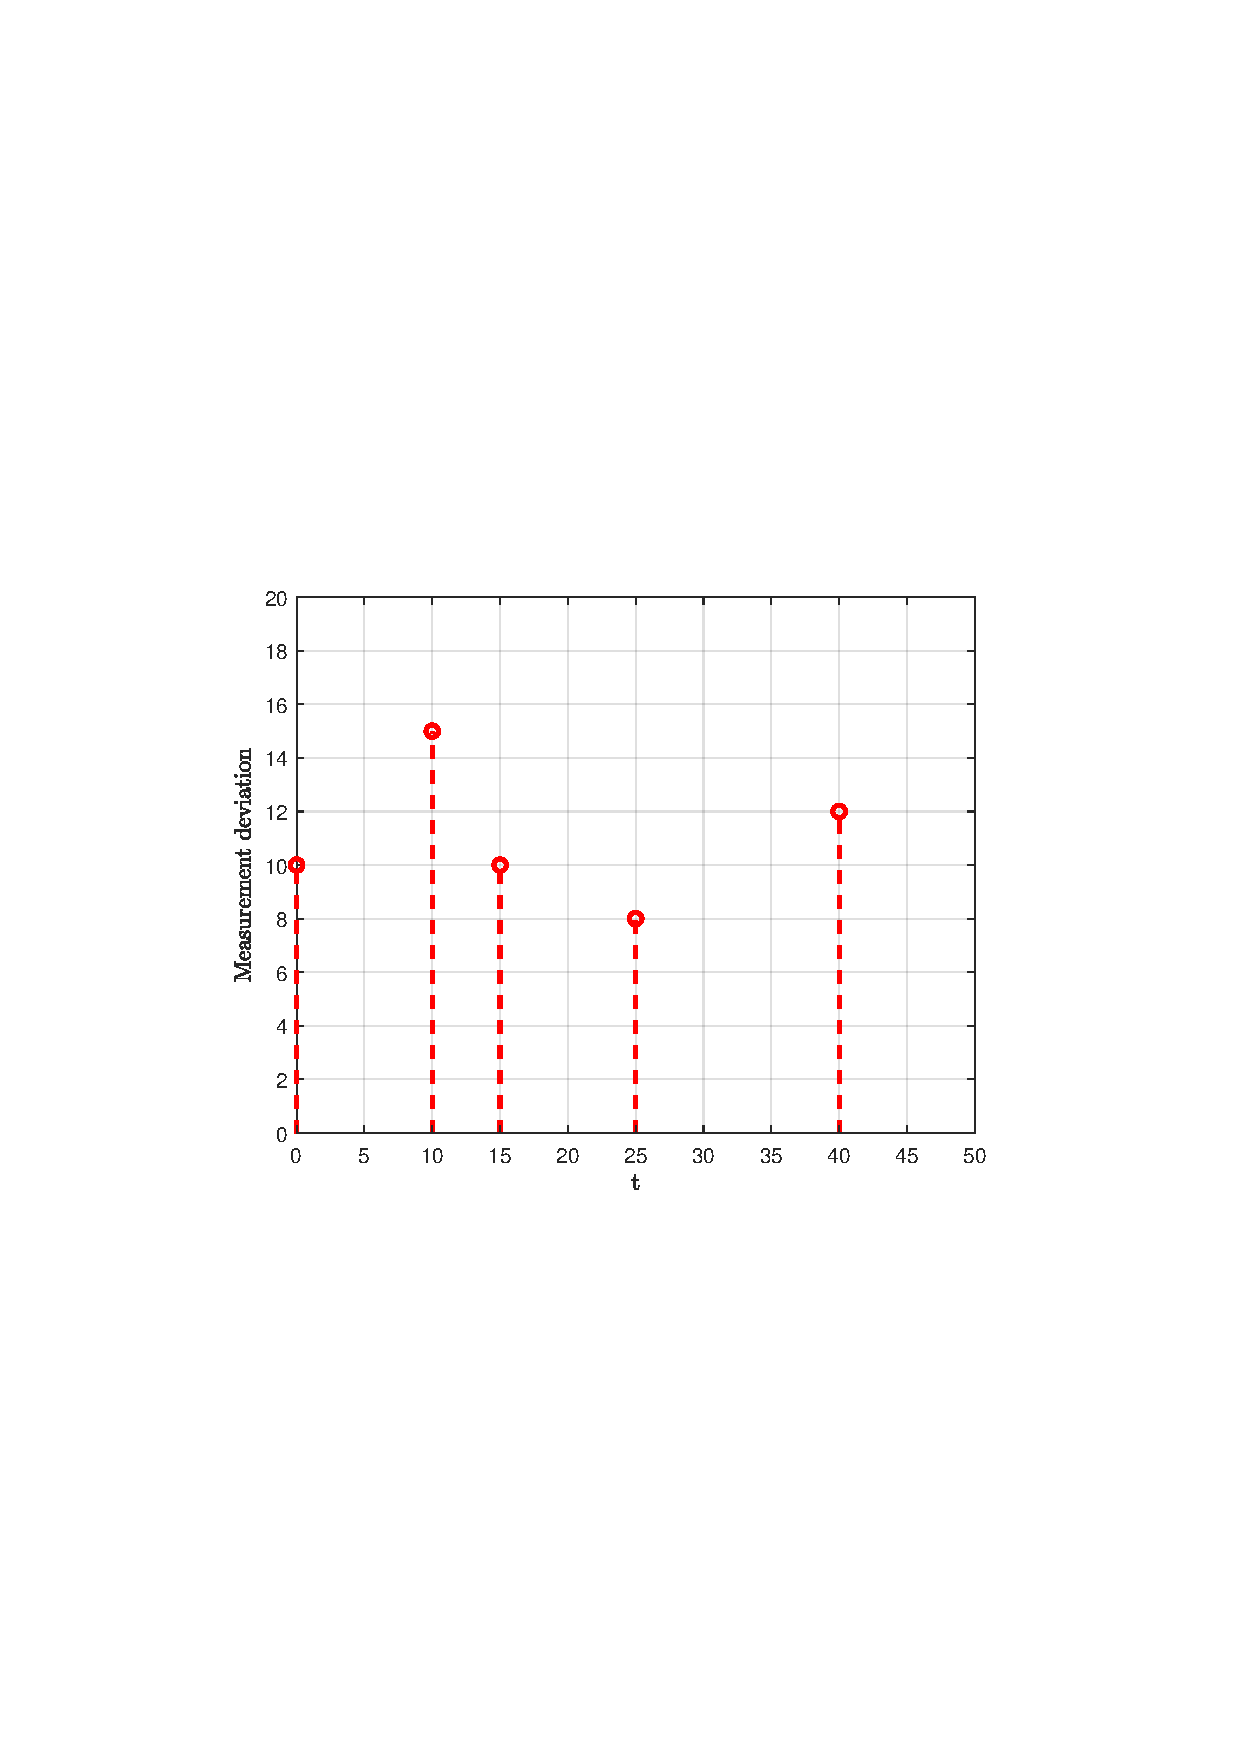
\includegraphics[width=3.5in]{outlier.pdf}
	\caption{\color{red}Measurement deviation caused by abnormal disturbance.}
	\label{Fig.4}
\end{figure}

Thank you once again for your valuable feedback regarding the relevant concepts in this paper. We hope that these revisions will improve the logical structure and coherence of the manuscript, making the connection between key concepts and related work clearer. Your suggestions will undoubtedly help enhance the presentation of the research.
~\\
\\
\textbf{2.} Authors are suggested to explain the framework presented in figure 1 in detail.
\\[10pt]
\begin{figure}[h]
	\centering
	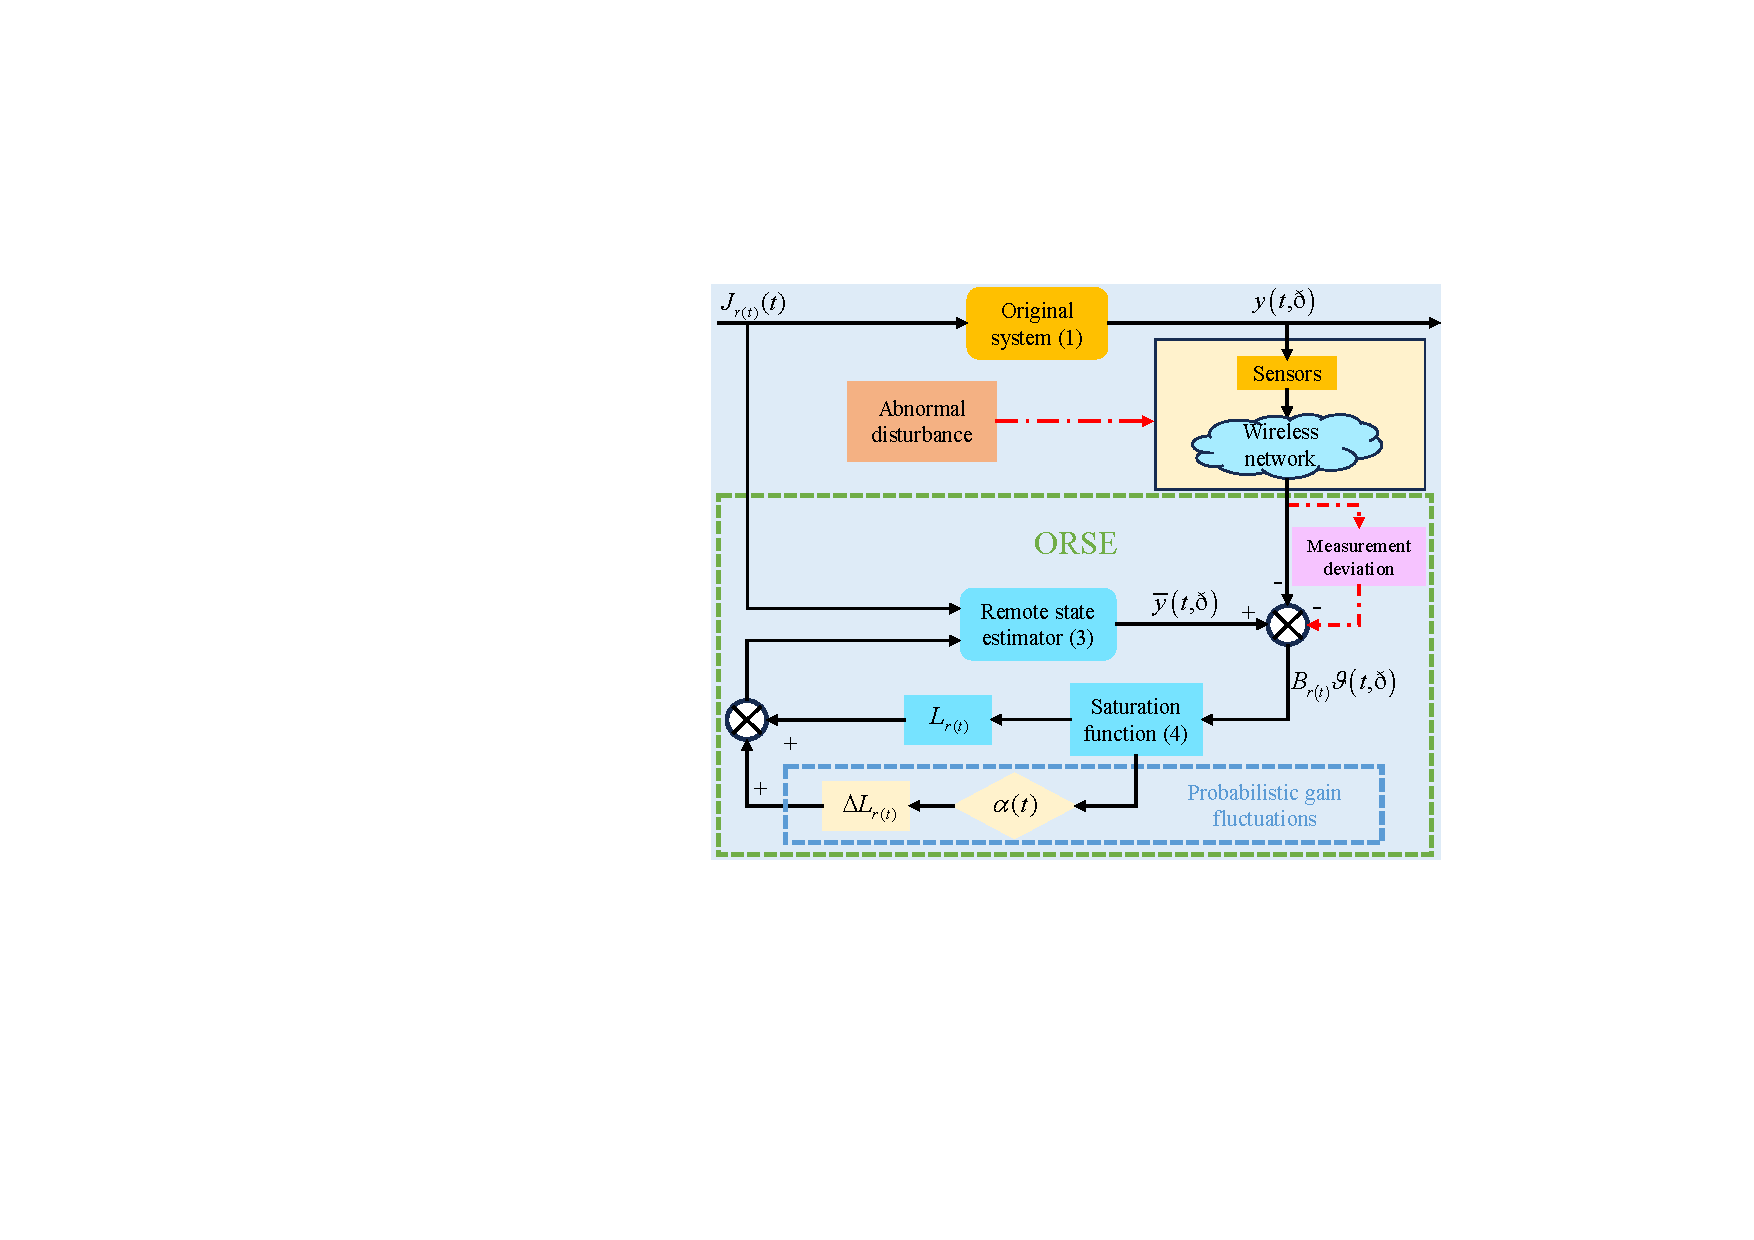
\includegraphics[width=3.5in]{ORSE.pdf} 
	\caption{{\color{red}The framework of the ORSE for semi-Markov switching RDNNs.}} 
	\label{Fig.1} 
\end{figure}

\indent \textbf{Reply 2:} Thank you very much for this constructive suggestion. We have revisited Fig. 1 and made the necessary revisions. A detailed explanation of Fig. 1 is as follows:\\

The framework illustrated in Fig. 1 corresponds to the model described in Section 2. The output $y(t,\eth)$ of the observed system (1) is measured by sensors and transmitted to the remote state estimator through a wireless network. The estimator then obtains the estimation error $B_{r(t)}\vartheta(t,\eth)$ between the estimator output $\bar{y}(t,\eth)$ and the measured data of the estimated system (1) output $y(t,\eth)$. It is worth noting that abnormal disturbances, such as sensor faults or network attacks, may cause the measured data $y(t,\eth)$ to become outliers that deviate significantly from their true values, thereby leading to abnormal estimation errors. The error signal is processed by a saturation function (4), which suppresses these outliers to the saturation boundary. Subsequently, the adjusted signal, combined with the probabilistically fluctuating estimator gain, is fed back into the estimator, enabling it to update the estimated state based on the processed error information.
~\\
\\
\textbf{3.} What are the advantages of considered asymmetric Lyapunov function when compared to conventional ones? What about the computational complexity?
\\[10pt]
\indent \textbf{Reply 3:} Thanks to you for your good comment. \\

Compared with the traditional LKF, the proposed asymmetric LKF offers two main advantages.\\

First, the matrix $R_2$ in the LKF $V_2(t)$ is not required to be symmetric, and when $R_2=0$, $V_2(t)$ naturally degenerates into the conventional LKF. Second, the proposed asymmetric LKF relaxes the positive definiteness constraint on all associated matrices, thereby reducing conservatism compared with traditional LKF. A detailed explanation of the proposed asymmetric LKF, along with an analysis of its computational complexity, is provided in Remark 3.1.\\

\textbf{Remark 3.1.} It is noteworthy that an important characteristic of $V_1(t, \eth)$ is its dependence on the system mode. In addition, unlike conventional LKFs, the constructed $V_2(t, \eth)$ is asymmetric. However, when $R_2 = 0$ in Theorem 3.1, $V_2(t, \eth)$ degenerates into a symmetric form. Moreover, the positive definiteness condition of this LKF is more relaxed compared to traditional LKF, requiring only the matrices $\Theta_{1}$, $\Theta_{2u}$, $T$ and $N D_k$ to be positive definite, without imposing positive definiteness on all related matrices, thereby reducing the conservatism in the analysis process. {\color{red} Furthermore, for the $u$th semi-Markov mode in Theorem 3.1, the number of decision variables is $n[8.5n+0.5(\mathcal{N}+1)( \mathcal{N}+2)n+(\mathcal{N}+10)n+5.5]$. It is worth noting that if $V_2(t, \eth)$ were replaced by a general symmetric augmented LKF of the form $V_2(t, \eth) = \int_\Omega \int_{t-\wp}^t \left[\vartheta^\text{T}(\nu, \eth), \int_\nu^t \vartheta^\text{T}(\mu, \eth) d\mu \right] R \left[ \vartheta^\text{T}(\nu, \eth), \int_\nu^t \vartheta^\text{T}(\mu, \eth) d\mu \right]^\text{T} d\nu \, d\eth$, where $R \in \mathbb{R}^{2n \times 2n}$ is positive define matrix, the resulting $V_2(t, \eth)$ would significantly increase the complexity of condition (12), thereby raising the computational complexity.}


~\\
\\
\textbf{4.} In simulation section, open-loop and closed-loop time profile of state estimation error trajectories are provided. What does open-loop and closed-loop refer here since it does not involve a feedback mechanism?\\

\indent \textbf{Reply 4:} Thank you for your suggestion. In the open-loop case, the estimator gain $L_{r(t)}=0$, which means that the error signal is not fed back to the estimator. Consequently, the estimator and the estimated system (1) operate as two independent systems. In contrast, the closed-loop case corresponds to a nonzero estimator gain, where the error signal is fed back through the gain to the estimator, enabling it to update the estimated state based on the estimated error. We have made additional clarifications in the simulation section as follows:\\

{\color{red}When the estimator gain $L_{r(t)}=0$, the system operates in an open-loop condition, where the error signal cannot be transmitted to the estimator, and systems (1) and (3) are independent of each other.} Fig.~5 shows the open-loop error trajectory, where the estimator fails to provide accurate estimation, resulting in noticeable estimation errors. In contrast, {\color{red}when the estimator gain $L_{r(t)} \neq 0$, the error system operates in a closed-loop condition, and the estimator updates the estimated state based on the error signal.} Fig.~6 presents the closed-loop state trajectory, where the error trajectory converges to zero.
~\\
\\
\textbf{5.} The modelling framework involves Bernoulli variables; therefore, is one simulation run enough to show the comparison results in Table 1?\\

\indent \textbf{Reply 5:} Thanks to you for your good comment.\\

Due to the presence of the Bernoulli variable, the fluctuation of the estimator gain differs in each simulation run, leading to variations in the comparative results shown in Table 1. This phenomenon is reasonable and expected. The results in Table 1 correspond specifically to the evolution of the Bernoulli random variable illustrated in Fig.~4. As long as the Bernoulli variable $\alpha(t)$ evolves as depicted in Fig.~4 with an expected value of 0.6, the results in Table 1 remain fixed. To further demonstrate the reliability of the comparison, several additional sets of results under different expectations $\bar{\alpha}$ have been added and are presented in Table 2 and Table 3.\\

\begin{table}[h]
	\centering
	{\color{red}
		\caption{{\color{red}The estimation error caused by measurement outliers with $\bar{\alpha}=0.5$.}}
		\label{tab2}
		\begin{adjustbox}{width=1\textwidth}
		\begin{tabular}{c|c|c|c|c|c}
			\toprule
			\multicolumn{2}{c|}{Time}& 10 & 15 & 25 & 40 \\ \hline
			\multicolumn{2}{c|}{Measurement outlier} &$y_i(10,0.5) + 15$ & $y_i(15,0.5)+10$ & $y_i(25,0.5)+8$ & $y_i(40,0.5)+12$ \\ \hline
			\multirow{2}*{Resilient state estimator}& $\vartheta_1(t,0.5)$ & 0.915 & 0.619 & 0.491 & 0.743 \\ \cline{2-6}
			~ & $\vartheta_2(t,0.5)$ & -0.186 & -0.135& -0.910 & -1.093 \\ \hline
			\multirow{2}*{ORSE} & $\vartheta_1(t,0.5)$ & 0.111 &0.113 & 0.112 & 0.113\\ \cline{2-6}
			~ & $\vartheta_2(t,0.5)$ & -0.165 &-0.166 & -0.165 & -0.166 \\ \bottomrule
		\end{tabular}
	\end{adjustbox}
	}
\end{table}

\begin{table}[h]
	\centering
	{\color{red}
		\caption{{\color{red}The estimation error caused by measurement outliers with $\bar{\alpha}=0.8$.}}
		\label{tab3}
		\begin{adjustbox}{width=1\textwidth}
		\begin{tabular}{c|c|c|c|c|c}
			\toprule
			\multicolumn{2}{c|}{Time}&10 & 15 & 25 & 40 \\ \hline
			\multicolumn{2}{c|}{Measurement outlier} &$y_i(10,0.5) + 15$ & $y_i(15,0.5)+10$ & $y_i(25,0.5)+8$ & $y_i(40,0.5)+12$ \\ \hline
			\multirow{2}*{Resilient state estimator}& $\vartheta_1(t,0.5)$& 0.919 & 0.214 & 0.168 & 0.746 \\ \cline{2-6}
			~ & $\vartheta_2(t,0.5)$ & -1.357& -0.126 & -0.100 & -1.095 \\ \hline
			\multirow{2}*{ORSE} & $\vartheta_1(t,0.5)$ & 0.112 & 0.072 & 0.070 & 0.113 \\ \cline{2-6}
			~ & $\vartheta_2(t,0.5)$ & -0.164 & -0.041 & -0.042 & -0.166 \\ \bottomrule
		\end{tabular}
	\end{adjustbox}
	}
\end{table}
~\\
\\
\textbf{6.} The author should provide the future direction in conclusions, which scenarios are going to be discussed in future.\\

\indent \textbf{Reply 6:} Thanks to you for your good comment. In response, we have expanded the conclusion section to discuss the future directions of this research. The specific points are as follows:\\

``Eventually, two numerical examples are presented to verify the effectiveness of the proposed theoretical methodology. {\color{red}In the future, we will consider the case of asynchronous switching between the estimator and system modes. Additionally, to further improve the estimation performance of outlier-resistant estimator, it will be necessary to enhance the estimator structure, such as by adopting a saturation function with dynamic thresholds."}(In the conclusion)
~\\
\\

Special thanks to you for your good comments. All your suggestions are very important, they have important guiding significance to my thesis writing and scientific research work.\\


Thank you for this constructive suggestion again!

~\\
\\
*****************************************************************************************\\
\\
\hspace*{-0.5cm}\indent\textbf{Reviewer $\sharp$ 2:}  This paper primarily centers on the H$\infty$ remote state estimation for reaction-diffusion neural networks with semi-Markov switching coefficients. An asymmetric Lyapunov-Krasovskii functional is constructed to alleviate the positive definiteness constraint and reduce conservatism, and then sufficient conditions of the asymptotic stability with prescribed H$\infty$ performance for the error system are derived. Overall, the work is well explained and organized. The authors may consider a few minor points.
\\
~\\
\textbf{1.} It is suggested that the authors highlight the innovation points of the paper and enrich the introduction of the paper, especially for the recent results on the neural networks, e.g, 10.1109/TNNLS.2019.2896162, and 10.1109/TCYB.2019.2908187.\\

\indent \textbf{Reply 1:} Thank you very much for your comment. In response to your suggestion, we have enriched the introduction to highlight the innovation and significance of our work, and have included relevant references.\\

``{\color{red}Compared with time-dependent switching mechanisms [12] and MJP, the semi-MJP exhibits higher randomness and generality, enabling a more accurate characterization of the stochastic and memory-dependent switching behaviors in practical systems [13, 14]."}(The second paragraph in the introduction)\\

``{\color{red}Therefore, investigating the design of outlier-resistant estimators to mitigate the impact of outliers on estimation performance is of significant importance. Although numerous results have been reported on estimator designs addressing outliers or gain perturbations, these approaches fail to simultaneously suppress the adverse effects of measurement outliers and probabilistic parameter fluctuations.} Based on the above discussions, designing an ORSE is essential to ensure the effectiveness of the estimator. According to our understanding of the existing literature, no existing research has addressed this issue for semi-Markov switching RDNNs, which constitutes one of the primary motivations for this study."(The fourth paragraph in the introduction)\\

{\color{red} [3] H.~Sang, J.~Zhao, Exponential {{Synchronization}} and {{L}}\_2 -{{Gain
			Analysis}} of {{Delayed Chaotic Neural Networks Via Intermittent Control With
			Actuator Saturation}}, IEEE Trans. Neural Netw. Learn. Syst. 30~(12) (2019)
	3722--3734.}\\
	
{\color{red} [12] H.~Sang, J.~Zhao, Sampled-{{Data-Based H}}{$\infty$} {{Synchronization}} of
	{{Switched Coupled Neural Networks}}, IEEE Trans. Cybern. 51~(4) (2021)
	1968--1980.}\\
	
Thank you for pointing out the deficiencies in the introduction section of the paper. We greatly appreciate your valuable feedback. We have made revisions to the manuscript, hoping that these changes will enhance the logical flow and coherence of the paper, and clarify the connection between key concepts and related work. Your suggestions will undoubtedly help strengthen the presentation of the research.

~\\
\\
\textbf{2.} Regarding the reaction-diffusion neural networks with semi-Markov switching coefficients, what is the difference if compared with that in 10.1109/TCSII.2022.3223938.
\\[10pt]
\indent \textbf{Reply 2:} Thank you very much for this constructive suggestion. The semi-Markov delayed RDNNs considered in this paper differs from the switched generalized delay neural network in 10.1109/TCSII.2022.3223938 in the following three aspects:\\

1) The neural network model in this paper is formulated using partial differential equations (PDEs), whereas the model in 10.1109/TCSII.2022.3223938 is based on ordinary differential equations (ODEs). This paper takes into account the reaction-diffusion phenomenon in neuron states, leading to a system described by PDEs involving both time and spatial variables. In contrast, the system equation in 10.1109/TCSII.2022.3223938 only relates to time variables. The modeling approach in this paper better aligns with real-world scenarios, especially when considering spatial dynamics.\\

2) The activation function term in the state equation differs between the two models. In this paper, the activation function term in the system model takes the form $Wf(\varsigma(t,\eth))$, while in 10.1109/TCSII.2022.3223938, the activation function term is $f(W\varsigma(t,\eth))$. Physically, the distinction lies in the order of processing: in the former, the neuron state is first nonlinearized by the activation function and then weighted, while in the latter, the neuron state is first weighted and then nonlinearized by the activation function. \\

3) The switching mechanism in this paper follows a semi-Markov process, where switching is random and the switching intervals exhibit memory. In contrast, the switching mechanism in 10.1109/TCSII.2022.3223938 is based on a combined switching strategy, where the switching time depends on both time and state, and the dwell time follows a fixed minimum dwell time.

~\\
\\
\textbf{3.} A procedure summarizing how implement in practice the proposed control strategy would improve the readability of the paper. Thus, an algorithm is suggested to minimize the H$\infty$ performance index $\gamma$.
\\[10pt]
\indent \textbf{Reply 3:} Thank you for this valuable suggestion. In response to this suggestion, we have provided a clear description of the algorithm for minimizing the H$\infty$ performance index $\gamma$ in Remark 3.4.\\

\textbf{Remark 3.4.}  {\color{red} The lower value of $\gamma$ indicates better capability in suppressing external disturbances and maintaining system stability. Therefore, minimizing the H$\infty$ performance index $\gamma$ is crucial in practical systems. Based on the results in Theorem 3.1, the optimization problem for minimizing the H$\infty$ performance index can be formulated as follows:
\begin{align*}
	\min \gamma \ \text{subject to} \, \Theta_{1}\textgreater 0,\, \Theta_{2u} \textgreater 0,\,  T \textgreater 0,\,  N D_k \textgreater 0, \, \hat{\Xi}_u  \textless 0
\end{align*}}

We believe that this addition enhances the readability and practical applicability of the paper by clarifying how to implement the proposed control and estimation framework in practice.
~\\
\\
\textbf{4.} In my opinion, an application to a practical system would increase the appeal of the paper. Is there a physical interpretation of the nonlinear function considered in the example?
\\[10pt]
\indent \textbf{Reply 4:} Thank you very much for your comment.  Regarding the physical interpretation of the nonlinear activation functions discussed in our paper, we provide the following explanation:\\

\textbf{Remark 2.5.}  {\color{red}The nonlinear functions are physically realized as input-output response circuits in hardware, where electronic components inherently exhibit nonlinear saturation characteristics [36]. For example, the activation function $f(\cdot)=\tanh(\cdot)$ exploits the natural saturation behavior of differential transistor pairs, causing the output voltage to smoothly saturate to the drain voltage. The saturation function (4) can be implemented by incorporating clamping diodes into the operational amplifier, which strictly restricts its output voltage to a specific saturation level within the power supply rails.}\\

We believe that these additional explanations provide a clearer physical and engineering interpretation of the nonlinearities in the proposed model, enhancing both the practical relevance and readability of this paper.
~\\
\\	
\textbf{5.} Please check the paper for typos.
\\[10pt]
\indent \textbf{Reply 5:} We appreciate the your careful reading and kind reminder. The entire manuscript has been thoroughly proofread to eliminate typographical and grammatical errors. Minor language corrections and formatting adjustments have been made throughout the paper to ensure accuracy and clarity.
~\\
\\
\textbf{6.} In conclusion part, more future works and challenges are recommended.
\\[10pt]
\indent \textbf{Reply 6:} Thanks to you for your good comment. In response, we have expanded the conclusion section to discuss the future directions of this research. The specific points are as follows: \\


``Eventually, two numerical examples are presented to verify the effectiveness of the proposed theoretical methodology. {\color{red}In the future, we will consider the case of asynchronous switching between the estimator and system modes. Additionally, to further improve the estimation performance of outlier-resistant estimator, it will be necessary to enhance the estimator structure, such as by adopting a saturation function with dynamic thresholds.}"(In the conclusion)\\

Special thanks to you for your good comments. All your suggestions are very important, they have important guiding significance to my thesis writing and scientific research work.\\


Thank you for this constructive suggestion again!\\


I wish you every success in your work!\\

Sincerely yours:
\\

\indent Xiaoqing Li\\

School of Electrical Engineering and Automation\\

Hefei University of Technology, Hefei 230009, China\\

\indent Oct.25, 2025.
\end{document}
